%!TEX root = document.tex


We define the social affinity between two users $u$ and $v$ via their direct {\em interactions}
on various digital items, and their {\em activities} in the different communities in the social network. 

\begin{figure}[t!]
\centering
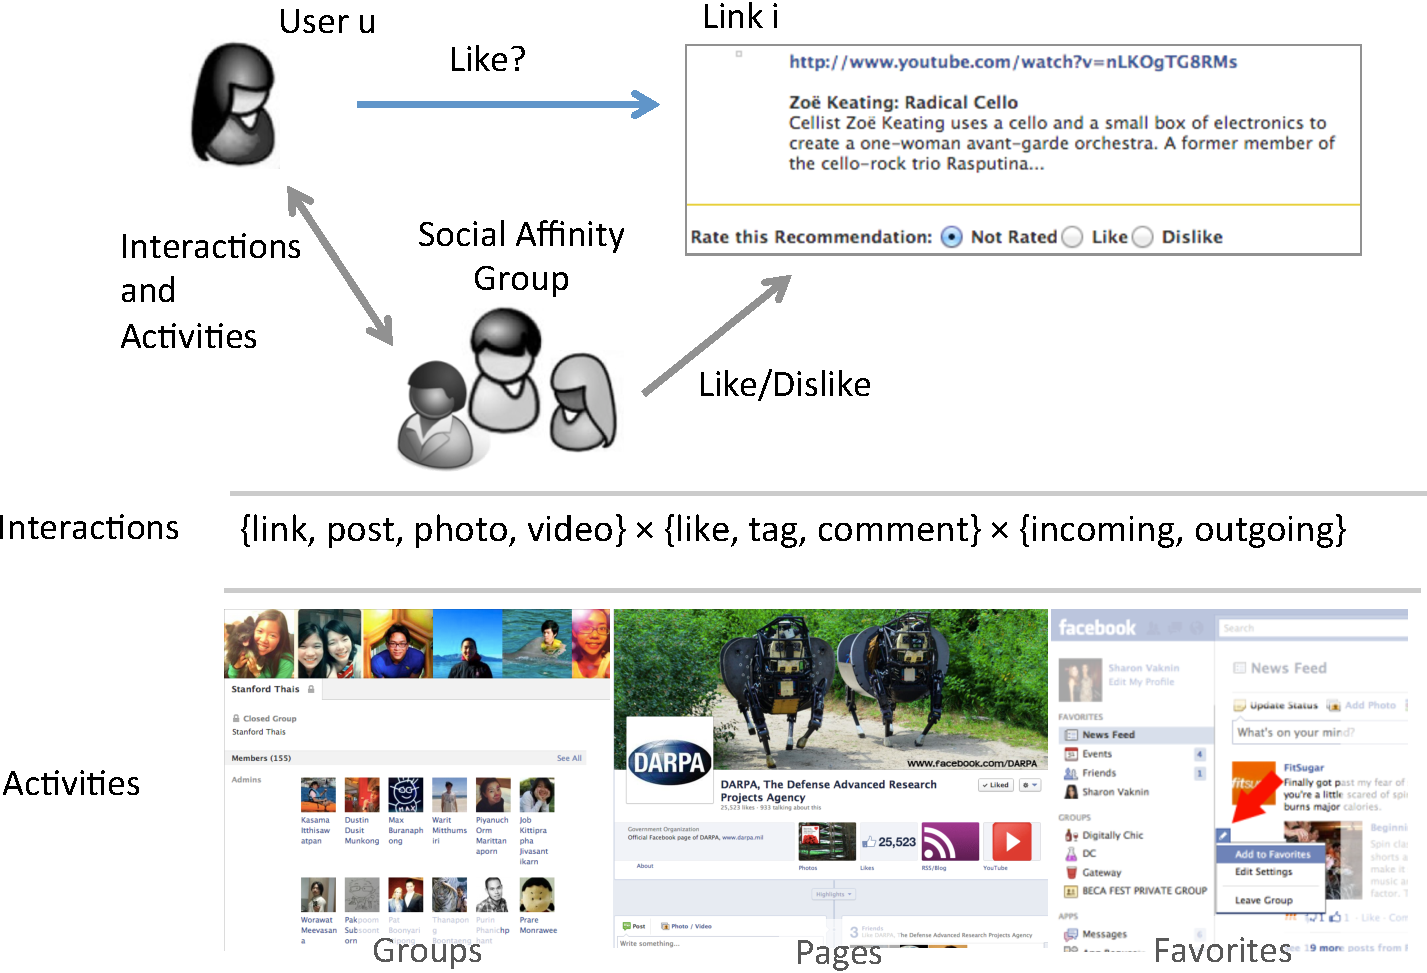
\includegraphics[width=.95\linewidth]{data/overview}
\caption{Overview of social affinity for link recommendation.}
\label{fig:overview}
\end{figure}


We categorize facebook user-user and user-entities relationship into two broad categories ie \textbf{Interactions} and \textbf{Activities}.

{\bf Interactions} describes the communication between Facebook users based on modality, action and direction.
\begin{itemize}
\item \textbf{Modality :}  User can interact with other users via
									 \textit{links, posts, photos} and \textit{videos}.
\item \textbf{Action :}  A user $u$ can \textit{comment} or \textit{like} 
									user $v$'s item or \textit{tag} user $v$ on an 
									item(with one exception in Facebook that $u$ cannot tag a 
									link with users $v$ for the obvious reason) .
\item \textbf{Directionality :} Motivated by~\cite{saez2011high}, we can look
      								at \textit{incoming} and \textit{outgoing} interactions, i.e.,
      								if user $u$ comments on, tags, or likes user $v$'s item,
      								then $u$ is in the set of incoming interactions for $v$
      								and $v$ is in the set of outgoing interactions for $u$.
      								
\end{itemize}								

%\subsection{Activities}
{\bf Activities} describes the user interactions with Facebook entities like groups, pages, favourite movies, favourite music etc.
\begin{itemize}
  %@SCOTT/LEXING following defination are taken from facebook blog. I am confused how to cite it %
  \item \textbf{Groups :} Facebook Groups are the place for small group communication and for people to share their common interests 
  						and express their opinion. Groups allow people to come together around a common cause, issue or activity to
  						organize, express objectives, discuss issues, post photos and share related content.
  \item \textbf{Pages :}  Facebook Pages enable public figures, businesses, organizations and other entities to create an authentic 
  						and public presence on Facebook. Facebook Pages are visible to everyone on the internet 
  						by default. Facebook user can connect with these Pages by becoming a fan and then receive their updates and interact with them.
  \item \textbf{Favourites :} Facebook facilitates a wide variety of user selected favourites (Activities, Favorite Athletes, Books, 
  							Interests, Movies, Music, Sports, Favorite Teams, Television ). These favourites allow a user to associate themselves with other people who share their same favourite tendencies.
\end{itemize} 

Note that the notion of affinity we adopt is based on direct user {\em actions}
% interactions
Our affinity
\cite{Panigrahy2012ubr}
\cite{Goel2012structure}
\cite{Wilson2012BSG}



The major objective of this paper is to evaluate the effectiveness of \textit{Social Affinity Filtering(SAF)} and fine grained 
analysis of the informativeness of Interactions and Activities.We divide our recommendation algorithm into two categories based 
on Interactions and Activities of target user's \textit{ Social Affinity Groups(SAG)} with target item, 
namely \textit{Interaction  Social Affinity Groups(ISAG)} and \textit{Activity Social Affinity Groups(ASAG)}.

\begin{itemize}
  \item \textbf{Interaction  Social Affinity Groups}: We define the set of interaction affinity classes based on 
  Interaction modality, action and direction as
  \begin{quote}
  \begin{math}
  	\textit{Interaction Affinity Classes} = \{link, post, photo, video\} \times \{like, tag, comment\} \times \{incoming, outgoing\}
  \end{math}
  \end{quote}
  %Additionally, we add friendship interaction affinity class. \\
  We define 
  \begin{quote}
  \textit{ISAG(u, i)} : set of the users who have interaction $i$ with user $u$.
  \end{quote}
   For example,
   \begin{quote}
   
   \textit{ISAG(u, link-like-incoming)} : set of all users who have liked link posted by user $u$. \\
   \textit{ISAG(u, link-like-outgoing)} : set of all users whose link is liked by user $u$. \\
   \end{quote}
\item \textbf{Activity Social Affinity Groups}: We define activity affinity groups based on group membership, page likes and user favourites.
	\begin{quote}
	\textit{ASAG(u, i)} : set of the users who share the entity $i$ (group, page, favourite) with user $u$.   
	\end{quote}
\end{itemize}
Finally, we define
\begin{quote}
\begin{math}
likes(u,i) =  \begin{Bmatrix}
	  True & \text{if user $u$ likes item $i$}\\
	  False & \text{otherwise}
	  \end{Bmatrix}
\end{math}
\end{quote}
\subsection{Social Affinity Features}
\begin{itemize}
  \item \textbf{Interaction Social Affinity Features} : We define Interaction affinity features for target user $u$ and item $i$ for ISAG's classes 
  $ \langle X_{1},X_{2}\ldots,X_{k}\rangle$ as
  \begin{quote}
  \begin{math}
   X_{k,u,i} = \begin{Bmatrix}
   		True & if\ \exists v\in ISAG(u,k) \wedge likes(v,i)\\ \\
   		False & otherwise
   \end{Bmatrix}
  \end{math}
  \end{quote}
  Additionally we add friend feature which encodes whether the target item $i$ is liked by friend or not.
  \item \textbf{Activity Social Affinity Features} : We define activity affinity features for target user $u$ and item $i$   \
  $ \langle X_{1},X_{2}\ldots,X_{k}\rangle$ as\\ \\
  \begin{math}
   X_{k,u,i} = \begin{Bmatrix}
   		True & if\ \exists\ v\in \ ASAG(u,k) \wedge likes(v,i)\\ \\
   		False & otherwise
   \end{Bmatrix}
  \end{math}
	In our analysis we use only those features(groups, pages and favourites) that is joined/liked by atleast one of our app user.
\end{itemize}

We train naive bayes, Logistic Regression(LR) and Support Vector Machine(SVM) model with affinity features.
Logistic Regression and SVM algorithm was implemented using \textit{LIBLINER} \cite{liblinear} package. 
We define Constant predictor as baseline predictor. Constant predictor predicts the most common outcome in our datase ie disliket.
We compare the performance of Social Affinity Filtering with the state of the art social collaborative filtering technique 
Social MatchBox(SMB)\cite{SMB}.

In real world social networks activity features grows very quickly as number of user in social network increases. This motivates the fine grained
analysis of informativeness of social affinity features. Furthermore, fine grained analysis of interactions helps to understand the nature of user-user 
interactions and its predictiveness in greater detail. Hence, for the analysis of activities and interactions we rank the features using
\textit{Conditional Entropy}. 
\textit{Conditional Entropy} is defined as
\begin{quote}
\begin{math}
H(Y|X=True) = \\-\sum_{y\in{(like,dislike)}} p(y|X$=$true)$ $log( p(y|X$=$true))
\end{math}
\end{quote}

With the data and methodology now defined including all dimensions of our analysis, we now proceed to an in-depth discussion of our findings.





 




